\documentclass[letterpaper, 10 pt, conference]{ieeeconf}  % Comment this line out if you need a4paper
%\documentclass[a4paper, 10pt, conference]{ieeeconf}   % Use this line for a4 paper
\IEEEoverridecommandlockouts                                    % This command is only needed if you want to use the \thanks command
\overrideIEEEmargins                                                 % Needed to meet printer requirements.

%In case you encounter the following error:
%Error 1010 The PDF file may be corrupt (unable to open PDF file) OR
%Error 1000 An error occurred while parsing a contents stream. Unable to analyze the PDF file.
%This is a known problem with pdfLaTeX conversion filter. The file cannot be opened with acrobat reader
%Please use one of the alternatives below to circumvent this error by uncommenting one or the other
%\pdfobjcompresslevel=0
%\pdfminorversion=4

% See the \addtolength command later in the file to balance the column lengths
% on the last page of the document

\usepackage{graphicx}    % for pdf, bitmapped graphics files
%\usepackage{epsfig}    % for postscript graphics files
\usepackage{mathptmx} % assumes new font selection scheme installed
\usepackage{times}        % assumes new font selection scheme installed
\usepackage{amsmath}  % assumes amsmath package installed
\usepackage{amssymb}  % assumes amsmath package installed
\usepackage{multirow}    % for aligning table column headers that span columns
\usepackage{booktabs}   % for better tables 

\title{\LARGE \bf Formation Control: A Centralized and Decentralized Approach}

\author{Ajay Ahir, Ben Philps and Sumaiyah Kola}

\begin{document}

\maketitle
\thispagestyle{empty}
\pagestyle{empty}

%%%%%%%%%%%%%%%%%%%%%%%%%%%%%%%%%%%%%%%%%%%%%%%%%%%%%%%%%%%%%%%%%%%%%%%%%%%%%%%%
\begin{abstract}
	
Multi-robot formations have proved useful in applications for exploration, surveillance and `search and rescue'. In such domains reliable global communication is not a guarantee. In this paper we implement a centralized and decentralized approach to multi-robot formation control that includes a reactive formation switching strategy. The robot formations successfully navigate through obstacle fields, tight corners and narrow corridors.

\end{abstract}
	
%%%%%%%%%%%%%%%%%%%%%%%%%%%%%%%%%%%%%%%%%%%%%%%%%%%%%%%%%%%%%%%%%%%%%%%%%%%%%%%%
\section{INTRODUCTION}
	
In application domains such as exploration, surveillance and `search and rescue', coordination and control mechanisms for multiple robots have been shown to provide cost effective and fault tolerant solutions \cite{c1}.

Inspired by the natural coordinated behavior of bird flocking and ant swarming, formation control of multiple robots can improve surveillance coverage by combining sensor readings from individual agents. The main objective is for multiple robots to traverse the environment while maintaining an explicitly specified spacing relationship between agents.

In this paper we provide a centralized behavior-based approach to formation control with a formation switching strategy. This solution relies on each agent transmitting and receiving information from a global controller. We also provide a fault-tolerant decentralized approach, adopting a message passing technique, suitable when communication is limited.

\subsection{BACKGROUND}
\label{background}

Balch and Arkin provide a behavior-based approach to formation control, dividing the task into behavioral components, referred to as `motor schemas' \cite{c2}. 

\subsubsection*{Motor Schemas}

Given the current sensor inputs and robot positions, each motor schema generates a vector $\vec{V}_s$ as a behavioral response. $\vec{V}_s$ indicates the direction and magnitude of desired movement. Motor schemas for goal navigation, static/dynamic obstacle avoidance and formation maintenance generate vectors $\vec{V}_{goal}$, $\vec{V}_{static\_obs}$, $\vec{V}_{dynamic\_obs}$ and $\vec{V}_{form}$, respectively. A gain value $g_s$ dictates the contribution of each schema to the overall behavior.

The overall behavioral response $\vec{V}$ is calculated by weighting each vector with its gain value then summing and normalizing the result. To overcome local minima, an additional schema generating noise  $\vec{V}_{noise}$ is included.

\subsubsection*{Formation Maintenance}
Each robot $R_i$, in position $P_{R_i}$, has a desired formation position $F_i$ from which $\vec{V}_{form}$ is defined:

\[\vec{V}_{form} = F_i - P_{R_i}\]

Different referencing schemes exist to find $F_i$. Unit-referencing computes the average $P_R$ as the center of the formation, Leader-referencing defines the formation relative to a leader robot's pose, and Neighbor-referencing defines each robot's position relative to a predefined neighbor.

The magnitude of $|\vec{V}_{form}|$ is determined by the distance between $P_{R_i}$ and $F_i$. Zones are defined around $F_{i}$ as seen in Fig. \ref{formation_zones}. 

Within the \textit{dead zone}, the robot is considered to be in formation and so $\vec{V}_{form} = \vec{0}$. Within the \textit{control zone}, the magnitude linearly increases from the inner edge. The magnitude at the outer edge of the \textit{control zone} is propagated throughout the \textit{ballistic zone}.

\begin{figure}[ht]
\centering
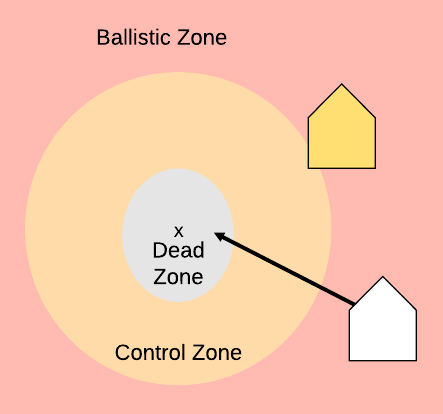
\includegraphics[width=0.45\linewidth]{images/formation_zones.png}
\caption{Zones for computing $\vec{V}_{form}$ with $F_i$ marked as `x'}
\label{formation_zones}
\end{figure}

\section{APPROACH}

We implement a Leader-referenced behavior-based approach to formation control. Additionally, we extend the work of Balch and Arkin to incorporate a formation switching strategy and a decentralized approach \cite{repository}.

A Leader-referenced approach allows the formation position of each robot to be determined with only knowledge of the leader $R_0$. 
In contrast, a Unit-referenced approach would require complete knowledge of all robot positions. Purely decentralizing this would require transmitting a substantial amount of state between robots.

We define motor schemas for goal navigation, obstacle avoidance and formation maintenance returning vectors $\vec{V}_{goal}$, $\vec{V}_{form}$ and $\vec{V}_{obs}$, respectively. Vectors from each schema are weighted and summed into an overall behavioral response $\vec{V}$ for each robot.

The addition of logical rules handles the avoidance of other robots in the centralized system where all robot poses are known.

\subsection{EXPERIMENTAL SET-UP}

We conduct experiments on 5 TurtleBot3 \cite{turtlebot} robots controlled using ROS \cite{ros} with Gazebo \cite{gazebo} as the simulation environment. We assume all robots are identical and labeled, with $R_0$ designated as leader and $R_1,...,R_n$ as followers. 

Each simulated robot is a non-holonomic differential-drive robot with control inputs $u$ and $\omega$, corresponding to linear and angular velocities, respectively. There are 5 sensors per robot, \texttt{right, front\_right, front, front\_left, left} evenly distributed around the front half of the robot.

We use feedback linearization to convert $\vec{V}$ into control inputs $u$ and $\omega$. This allows us to assume control of each robot via a holonomic point held at a distance of $\epsilon$. Here $\epsilon$ is 0.2m.

% TODO: figure out what our evaluation is doing and then do this scentence.
% to do need to amend this if our final impl doesnt do this! i.e. are we talking about all these? probs not
Our evaluation considers the performance of robot formations in multiple arenas that include obstacles, narrow corridors and tight corners. Fig. \ref{corridorworld} illustrates one of the testing arenas.

\begin{figure}[thpb]
\centering
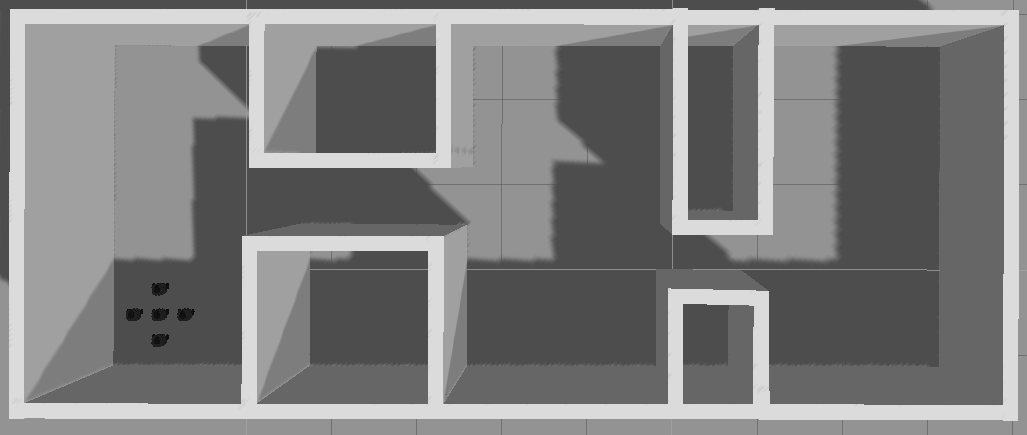
\includegraphics[width=\linewidth]{images/corridorworld.png}
\caption{The \textit{diamond} formation in an arena with tight corridors}
\label{corridorworld}
\end{figure}

\subsection{FORMATIONS}

We consider the following formations for 5 robots: \textit{diamond}, \textit{column}, \textit{line} and \textit{wedge} (Fig. \ref{formation_shapes}). Each formation is defined relative to the leader. The number of robots per formation and the intra-formation distance between robots can easily be adjusted to suit the environment.

\begin{figure}[thpb]
\centering
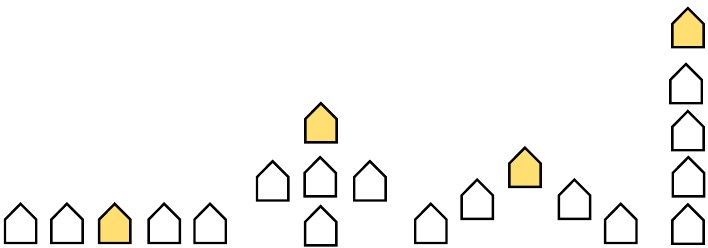
\includegraphics[width=0.7\linewidth]{images/formation_shapes.jpg}
\caption{Formations L-R: \textit{line}, \textit{diamond}, \textit{wedge}, \textit{column} with leader colored}
\label{formation_shapes}
\end{figure}

\subsection{MOTOR SCHEMAS}

The objective of the leader, $R_0$, is to reach the goal, avoiding obstacles and other robots. The objective of the followers, $R_1,...,R_n$, is to maintain formation while avoiding obstacles. 

Each motor schema has an associated gain value (Table \ref{motor_schema_gs}). The values were tuned empirically. Prioritizing obstacle avoidance above formation maintenance permits the desired split and merge behavior (see \textit{Obstacle Avoidance}).

Consequently, the behavioral response $\vec{V}$ for robot $R_i$ is:
\begin{equation*}
\begin{aligned}
\vec{V} = & g_{goal} \vec{V}_{goal} + g_{obs} \vec{V}_{obs} + \vec{V}_{noise}    && \text{if $R_0$} \\
              & g_{form} \vec{V}_{form} + g_{obs} \vec{V}_{obs} + \vec{V}_{noise}   && \text{if $R_1,...,R_n$}
\end{aligned}
\end{equation*}

where $\lvert\vec{V}_{noise}\rvert = 0.05$.

\begin{table}[h]
\begin{center}
\begin{tabular}{|c|cl|}
\hline
Motor Schema &  & Value \\
\hline
Goal Navigation & $g\_goal$                  & 0.35 \\
Obstacle Avoidance & $g\_obs$     & 0.22 \\
Formation Maintenance & $g\_form$       & 0.20 \\
\hline
\end{tabular}
\end{center}
\caption{Motor Schema Gain Values $g_s$}
\label{motor_schema_gs}
\end{table}

\subsubsection*{Goal Navigation}

$\vec{V}_{goal}$ points from $R_0$ to the next point along a path from $P_{R_0}$ to the goal. $\vert \vec{V}_{goal} \rvert = 1$.

We generate a path using an optimized version of the rapidly-exploring random trees (RRT) algorithm, RRT*. RRT* efficiently explores the search space by building a space-filling tree. Additional rewiring and cost minimization steps can generate an approximate shortest path to the goal. 

\subsubsection*{Obstacle Avoidance}
\label{subsubsection: obs avoid}

% todo sort this entire paragraph out
For the centralized system a Braitenberg controller was adopted. Since robots can detect each other on their sensors, the sensors are filtered. Where robot $R_B$ is in front of a sensor on robot $R_A$, and there is no obstacle detected between the robots, $R_A$'s sensor value is set to its maximum measurement.
The highest priority is given to the \texttt{front\_left} and \texttt{front\_right} sensors. When turning away from obstacles, robots determine a preferred direction proportional to each smoothed sensor measurement and its position in the formation. This allows the robots to split and merge efficiently, avoiding robots crossing paths. This also encourages wider exploration of the environment.
Filtering robot positions from sensor methods is not possible in the decentralized system. A rule-based system designed to function more smoothly when robots are detected by the sensors was implemented.
Both controllers return a vector $V\_obs$.
%todo: what are the magnitudes for these controllers

\subsubsection*{Formation Maintenance}

We use the implementation of this motor schema defined in Balch and Arkin and described in \ref{background}. 

To calculate $F_i$ we transform the vector of relative formation positions, by rotating it to match the leader's orientation then translating it to the leader's position.

We normalize $V_{form}$ by calculating $V_{form}/|control\_zone|$. Table \ref{table_formation} contains the parameters used to implement this motor schema.

\begin{table}[h]
\begin{center}
\begin{tabular}{|c|c|c|}
\hline
& Parameter & Value (m) \\
\hline
(1) & Robot Radius             & 0.05 \\
(2) & Spacing Distance        & 0.8 \\
(3) & Dead Zone Radius      & $1.5 \times (1) = 0.075$ \\
(4) & Control Zone Radius    & (2) $+$ (3) $=0.875$ \\
\hline
\end{tabular}
\end{center}
\caption{Formation Maintenance Parameters}
\label{table_formation}
\end{table}

When follower robots are not in their dead zone, $g_goal$ is decreased, so that the leader waits for the followers to catch it.
%TODO add switch formation for goal heuristic

\subsection{Dynamic Obstacle Avoidance}

Dynamic obstacle avoidance applies to other robots. We produce a weight vector $W$ which takes value $0$ to tell robot $R_i$ to stop moving if it is behind robot $R_j$, and is $1$ otherwise. If the two robots are approximately adjacent then the robot with the lowest ID stops and the other moves to avoid deadlock. The weight is computed based on the distance between robots and how much they face each other.


\subsection{FORMATION SWITCHING STRATEGY}

We implement a reactive formation switching strategy. This determine the safest formation for the robots, given the current environment

If the leader, or at least half of the followers, detect a corridor, the formation is switched to a \textit{column}.
This formation is maintained until the robots exit the corridor, at which point it is safe to return to the default formation. We chose \textit{column} as it is the narrowest formation.

A robot is said to `detect' a corridor if the environment ahead of the \textit{front} sensor is clear and the \textit{left} and \textit{right} sensors report measurements below a threshold, here 0.4m.

\subsection{DECENTRALIZED}

The centralized algorithm relies on knowledge of all robot positions as well as their combined view of the world. Our decentralized solution achieves this with limited message passing between robots to communicate the required state. Communication links are defined between certain robots in each formation. For \textit{line}, \textit{column} and \textit{wedge}, links are defined between adjacent robots. For \textit{diamond}, all robots are arranged so they can communicate with the center robot.

Our consensus algorithm uses each robot's ID to decide the leader. Robot $R_i$ is the leader if,
\[\text{form\_pos}[ID(R_i)] = (0,0)\]
Where `form\_pos' is the vector of relative formation positions and `$ID$' returns a robot's ID. IDs are assigned so that each corresponds to a unique position, such as by generating a random number and taking the next $n$ for $n$ robots. Only the leader initiates message passing when their state updates, and the other robots relay this message down their formation links, excluding the receiving link.

Decentralized obstacle avoidance is slightly different to centralized obstacle avoidance. The Braitenberg hybrid controller uses the additional knowledge of every other robot to compute which side of the formation a robot is on. As we do not have this state in the decentralized approach, we only use a rule-based controller limited to each robot.

\section{RESULTS}
% todo mention error is euclidian distnace
Visually our solution in both the centralized and decentralized case achieves formation control as seen by the sequence of images in Fig. X and Fig. Y. In order to quantify our results, we evaluate the performance by the error to the desired position for each robot,
\[err = |P_{desired} - P_{R_i}|\]
This acts as a measure for how out of formation robot $R_i$ is.

% TODOS
1) keep formation, successfully change formation, split and merge,
tight corners?
2) decentralized works too, but works better when spacing distances are sufficiently large so that robots don't effect sensors.
3) edit error plots
4) fill out tables (change them),
exploration (better with split and merge)
5) add units to the graph

% TODO:NAME arena.
% TODO: write this up properly.
% TODO: make sure earlier work in the paper reflects what we say here
% TODO: plots
% TODO: rigourous evaluation i.e. mention specific points on the curves
	

\begin{table}[t]
\begin{tabular}{@{}cp{1.75cm}cp{1.5cm}p{1.75cm}cp{1.5cm}@{}}
\toprule
\multicolumn{1}{l}{} & \multicolumn{1}{l}{}   & Centralized        & \multicolumn{1}{l}{}      & \multicolumn{1}{l}{}   & Decentralized      & \multicolumn{1}{l}{}      \\ \midrule
Formation            & Time to Reach Goal (s) & Position Error (m) & Time out of Formation (s) & Time to Reach Goal (s) & Position Error (m) & Time out of Formation (s) \\
\textit{line}        &                        &                    &                           &                        &                    &                           \\
\textit{column}      &                        &                    &                           &                        &                    &                           \\
\textit{diamond}     &                        &                    &                           &                        &                    &                           \\
\textit{wedge}       &                        &                    &                           &                        &                    &                           \\ \bottomrule
\end{tabular}
\caption{Performance of Robots in the Square Arena}
\label{tab:results_square}
\end{table}

\begin{table}[t]
\begin{tabular}{@{}cp{1.75cm}cp{1.5cm}p{1.75cm}cp{1.5cm}@{}}
\toprule
\multicolumn{1}{l}{} & \multicolumn{1}{l}{}   & Centralized        & \multicolumn{1}{l}{}      & \multicolumn{1}{l}{}   & Decentralized      & \multicolumn{1}{l}{}      \\ \midrule
Formation            & Time to Reach Goal (s) & Position Error (m) & Time out of Formation (s) & Time to Reach Goal (s) & Position Error (m) & Time out of Formation (s) \\
\textit{line}        &                        &                    &                           &                        &                    &                           \\
\textit{column}      &                        &                    &                           &                        &                    &                           \\
\textit{diamond}     &                        &                    &                           &                        &                    &                           \\
\textit{wedge}       &                        &                    &                           &                        &                    &                           \\ \bottomrule
\end{tabular}
\caption{Performance of Robots in the Corridor Arena}
\label{tab:results_square}
\end{table}

\section{CONCLUSION}

\addtolength{\textheight}{-12cm}   % This command serves to balance the column lengths
                                               % on the last page of the document manually. It shortens
                                               % the textheight of the last page by a suitable amount.
                                               % This command does not take effect until the next page
                                               % so it should come on the page before the last. Make
                                               % sure that you do not shorten the textheight too much.

%%%%%%%%%%%%%%%%%%%%%%%%%%%%%%%%%%%%%%%%%%%%%%%%%%%%%%%%%%%%%%%%%%%%%%%%%%%%%%%%
\section{ACKNOWLEDGMENT}

\begin{itemize}
\item Ajay Ahir - Worked on setting up the multi-robot environment and obstacle avoidance. Added the RRT* component and worked on combining velocities. Decentralized the solution and produced the error plots.

\item Ben Philps - 

\item Sumaiyah Kola - 
\end{itemize}

%%%%%%%%%%%%%%%%%%%%%%%%%%%%%%%%%%%%%%%%%%%%%%%%%%%%%%%%%%%%%%%%%%%%%%%%%%%%%%%%
\begin{thebibliography}{99}
	
\bibitem{c1} J. S. Jennings, G. Whelan and W. F. Evans, ``Cooperative Search and Rescue with a Team of Mobile Robots'', 8th International Conference on Advanced Robotics, Proceedings ICAR'97, Monterey, CA, USA, pp. 193-200, Jul. 1997.

\bibitem{c2} T. Balch and R. C. Arkin, ``Behavior-based Formation Control for Multi-robot Teams'', IEEE Transactions on Robotics and Automation, vol. 14, no. 6, pp. 926-939, Dec. 1998.

\bibitem{turtlebot} TurtleBot3, http://emanual.robotis.com/docs/en/platform/turtlebot3/overview/
\bibitem{ros} ROS - Robot Operating System, https://www.ros.org/
\bibitem{gazebo} Gazebo, http://gazebosim.org/
\bibitem{repository} Code Repository, https://github.com/DoodleBobBuffPants/RobotProject

\end{thebibliography}

\end{document}
